\documentclass{sigchi}

% Use this section to set the ACM copyright statement (e.g. for
% preprints).  Consult the conference website for the camera-ready
% copyright statement.

% Copyright
\CopyrightYear{2016}
%\setcopyright{acmcopyright}
\setcopyright{acmlicensed}
%\setcopyright{rightsretained}
%\setcopyright{usgov}
%\setcopyright{usgovmixed}
%\setcopyright{cagov}
%\setcopyright{cagovmixed}
% DOI
\doi{http://dx.doi.org/10.475/123_4}
% ISBN
\isbn{123-4567-24-567/08/06}
%Conference
\conferenceinfo{UIST'18,}{May 07--12, 2016, San Jose, CA, USA}
%Price
\acmPrice{\$15.00}

% Use this command to override the default ACM copyright statement
% (e.g. for preprints).  Consult the conference website for the
% camera-ready copyright statement.

%% HOW TO OVERRIDE THE DEFAULT COPYRIGHT STRIP --
%% Please note you need to make sure the copy for your specific
%% license is used here!
% \toappear{
% Permission to make digital or hard copies of all or part of this work
% for personal or classroom use is granted without fee provided that
% copies are not made or distributed for profit or commercial advantage
% and that copies bear this notice and the full citation on the first
% page. Copyrights for components of this work owned by others than ACM
% must be honored. Abstracting with credit is permitted. To copy
% otherwise, or republish, to post on servers or to redistribute to
% lists, requires prior specific permission and/or a fee. Request
% permissions from \href{mailto:Permissions@acm.org}{Permissions@acm.org}. \\
% \emph{CHI '16},  May 07--12, 2016, San Jose, CA, USA \\
% ACM xxx-x-xxxx-xxxx-x/xx/xx\ldots \$15.00 \\
% DOI: \url{http://dx.doi.org/xx.xxxx/xxxxxxx.xxxxxxx}
% }

% Arabic page numbers for submission.  Remove this line to eliminate
% page numbers for the camera ready copy
% \pagenumbering{arabic}

% Load basic packages
\usepackage{balance}       % to better equalize the last page
\usepackage{graphics}      % for EPS, load graphicx instead 
\usepackage[T1]{fontenc}   % for umlauts and other diaeresis
\usepackage{txfonts}
\usepackage{mathptmx}
% \usepackage[pdflang={en-US},pdftex]{hyperref} なんかわからない
\usepackage{color}
\usepackage{booktabs}
\usepackage{textcomp}

% Some optional stuff you might like/need.
\usepackage{microtype}        % Improved Tracking and Kerning
% \usepackage[all]{hypcap}    % Fixes bug in hyperref caption linking
\usepackage{ccicons}          % Cite your images correctly!
% \usepackage[utf8]{inputenc} % for a UTF8 editor only

% If you want to use todo notes, marginpars etc. during creation of
% your draft document, you have to enable the "chi_draft" option for
% the document class. To do this, change the very first line to:
% "\documentclass[chi_draft]{sigchi}". You can then place todo notes
% by using the "\todo{...}"  command. Make sure to disable the draft
% option again before submitting your final document.
\usepackage{todonotes}

% Paper metadata (use plain text, for PDF inclusion and later
% re-using, if desired).  Use \emtpyauthor when submitting for review
% so you remain anonymous.
\def\plaintitle{Bridging the Translation Gap with ExpandHelp}
\def\plainauthor{First Author, Second Author, Third Author,
  Fourth Author, Fifth Author, Sixth Author}
\def\emptyauthor{}
\def\plainkeywords{Authors' choice; of terms; separated; by
  semicolons; include commas, within terms only; required.}
\def\plaingeneralterms{Documentation, Standardization}

% llt: Define a global style for URLs, rather that the default one
\makeatletter
\def\url@leostyle{%
  \@ifundefined{selectfont}{
    \def\UrlFont{\sf}
  }{
    \def\UrlFont{\small\bf\ttfamily}
  }}
\makeatother
\urlstyle{leo}

% To make various LaTeX processors do the right thing with page size.
\def\pprw{8.5in}
\def\pprh{11in}
\special{papersize=\pprw,\pprh}
\setlength{\paperwidth}{\pprw}
\setlength{\paperheight}{\pprh}
\setlength{\pdfpagewidth}{\pprw}
\setlength{\pdfpageheight}{\pprh}

% Make sure hyperref comes last of your loaded packages, to give it a
% fighting chance of not being over-written, since its job is to
% redefine many LaTeX commands.
\definecolor{linkColor}{RGB}{6,125,233}
% \hypersetup{%
%   pdftitle={\plaintitle},
% % Use \plainauthor for final version.
% %  pdfauthor={\plainauthor},
%   pdfauthor={\emptyauthor},
%   pdfkeywords={\plainkeywords},
%   pdfdisplaydoctitle=true, % For Accessibility
%   bookmarksnumbered,
%   pdfstartview={FitH},
%   colorlinks,
%   citecolor=black,
%   filecolor=black,
%   linkcolor=black,
%   urlcolor=linkColor,
%   breaklinks=true,
%   hypertexnames=false
% }

% create a shortcut to typeset table headings
% \newcommand\tabhead[1]{\small\textbf{#1}}

% End of preamble. Here it comes the document.


\def\GH{\textsf{GitHelp}}

\begin{document}

\title{\plaintitle}

\numberofauthors{3}
\author{%
  \alignauthor{Toshiyuki Masui
    \affaddr{Keio University}\\
    \affaddr{Fujisawa, Japan}\\
    \email{masui@pitecan.com}}\\
  \alignauthor{Jun Kato\\
    \affaddr{AIST}\\
    \affaddr{Tsukuba, Japan}\\
    \email{junkato}}\\
}

\maketitle

\begin{abstract}
  We introduce a flexible command translation system that can generate
  a complex command string from vague keywords
  given by the user.
  %
  % Although intuitive GUI are 
  % command-line interface (CLI) is stil widely used everywhere,
  %
  When people use computers to perform tasks,
  there is usually a huge mismatch between the users' intention
  and the required action.
  % the language and vocabularies used for the task are completely different.
  When a user wants to ``make the room darker'',
  he should translate it to a real action like ``turn off the ceiling light''.
  To do so,
  he may have to ``toggle the wall switch''
  or issue a command like ``\texttt{\$ iot ceilinglight 0}''.
  If the user is a Chinese speaker, he might have to translate his intention
  ``使房黒暗'' into ``make the room darker'',
  translate it to ``turn off the ceiling light'', 
  and finally generate a command string like ``\texttt{\$ iot ceilinglight 0}''.

  People are perpetually suffering from such multi-level ``\textit{translation gaps}''.
  Translation gaps exist even for experienced computer users, but
  they are serious for vast amount of people around the world.
  %
  We propose a simple and general translation framework
  \textsf{ExpandHelp} that can be used in a wide area of situations
  where such translation is required.
  We show how our framework can be used
  in the {\GH} system
  with which user can easily generate complex \texttt{git} commands
  from fragments of users' intentions.

\end{abstract}

\category{H.5.m.}{Information Interfaces and Presentation
  (e.g. HCI)}{Miscellaneous} \category{See
  \url{http://acm.org/about/class/1998/} for the full list of ACM
  classifiers. This section is required.}{}{}

\keywords{\plainkeywords}

\section{Introduction}

When we use modern artifacts,
we shoule translate our intentions into actions required for the artifacts.
When we want to watch a movie, we may pick up a DVD disk, put it into a
DVD player, push the play button, and set up the audio and the monitor.
When we feel thirsty, we may go to the kitchen, pick up a glass, and
turn the faucet on to fill the glass with water.
All the living creatures seem to be performing such translations
between intentions and actions without difficulty, but
in the modern world, people are suffering from
serious gaps between what they want to do and what they have to do.

Even when people almost know what they have to do for what they want to do,
it is often not easy to perform the task properly.
Even when people know that they can watch a movie on the Internet,
finding a movie and playing it is a difficult task for people without experiences.
% even when detailed user manuals and documents exist.
It would be nicer if they could watch a movie on the net
just by showing a vague title or attributes of the movie
in various languages.

% We can use search engines to find clues for performing the tasks, but
% it is not always easy for people in the world, since they may have
% to use different languages to look for the information.

We propose a command translation system with which users can generate a complete
command string.
%
We provide a database consisting of
pairs of
(1) the description of the task that users want to perform,
and
(2) the actual command string required by the system.
(1) can be written using regular expressions in any language,

For example, the database can include data like
\texttt{\[ heya wo kuraku suru, \% iot ceiling 0 \]}.





% やりたいことの[* 平易な表現と実行コマンドの組を用意]して[* 共有]しておいて、[* 簡単に検索/実行]できるようにする
% 表現は[* 何語で書いてあってもかまわない]
% 例えば映画作品見たいならAmazon PrimeとNetflix両方に作品があったりする
% コマンドの例でいえば何をどの順番でパイプするかいろいろ選択肢がありうる
% 全部出てくれると便利ですね(自分の知らなかったコマンド記法が学べたりする)
% いろんな候補は出ます [増井俊之.icon]
% 「Amazonでゴジラを見る」「Netflixでゴジラを見る」みたいに
% コマンドの勉強になる とは思っています [増井俊之.icon]
% そういう話は記述した方がいいかも
% `@{2 days ago}`なんて記法を知ってる人は見たことなし [増井俊之.icon]
% 今は自力で打てるようになった!
% これを[* IMEみたいなインタフェースで利用する]
% ちなIMEはアジアでは常識ね
% [* データはWikiで共有しておいて誰でも追加/修正できる]
% 自分のやり方を定義してもいい

Contributions of this paper are as follows:

\begin{enumerate}
% 各種技術を組み合わせた翻訳支援というパラダイムの提案
\item Introduction of a ``translation paradigm'' to control a machine from vague specifications
\item IME-like command etnry system
% やりたいことを実行するインタフェース (IME的なもの)
\item Flexible dynamic search system based on RegExp (ExpandHelp)
% そのための柔軟なインフラ (ExpandHelp)
\item Data sharing infrastructure for the translation paradigm
% 共有/編集しやすい正規表現DSLとそのインプリ(Scrapbox+)
% \item これが唯一の解決法ではないが、こういう考え方がポピュラーになって欲しい
\end{enumerate}

\section{Example}

We have implemented the \textsf{GitHtlp} system
with which a user can translate his vague intention in various languages
into a complete \texttt{git} commands
using the \textsf{ExpandHelp} framework.

\paragraph{Entering a command}

We assume that the user is using \texttt{bash} for his software
development activities.

\begin{figure}[b]
  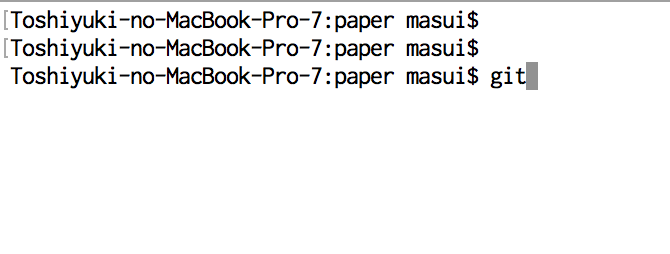
\includegraphics[width=8cm,bb=0 0 670 254]{figures/bash1.png}
  \caption{Bash shell.}
  \label{bash1}
\end{figure}

When the user wants to compare the latest \texttt{README.md} file with an
older version, he tries to use \texttt{git} to show the difference.
He may know that he can use the \texttt{git diff} command to do the
conparison and invoke the following command like the following.

\begin{quotation}
  \begin{verbatim}
    $ git diff README.md
    $
  \end{verbatim}
\end{quotation}

Nothing happens, because this is not the right command
to compare the latest version with older version.
%
More experienced user might use a command like the following,
but it does not show anything either, because the version specification
``\verb|HEAD^^|''
points at a file included in the older ``commit'',
and 

\begin{quotation}
  \verb|$ git diff HEAD^^ README.md|
\end{quotation}

If {\GH} is installed,
the user can type a special key (e.g. \texttt{Cmd-Ctrl-G}) to invoke {\GH}
after typing ``\texttt{git RE 2}''.

\begin{figure}[b]
  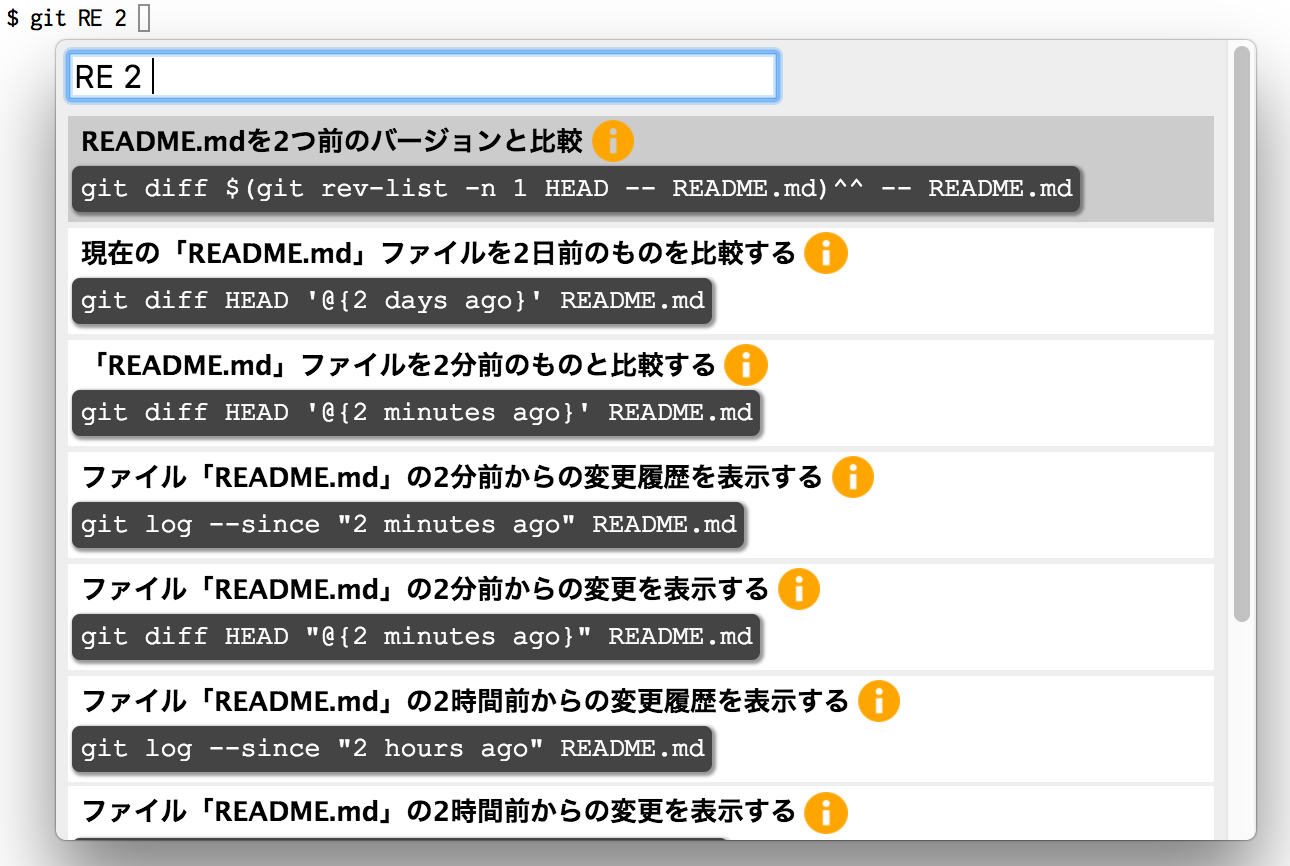
\includegraphics[width=8cm,bb=0 0 1290 866]{figures/githelp1.png}
  \caption{Invoking {\GH}.}
  \label{bash1}
\end{figure}

Here, various candidate entries with
descriptios and command strings are listed.
One of the entries says ``.....'',
which means that ``to compare README with two older verson.''
%
If the user thinks that that's what he wanted to do,
he can select the entry by typing arrow keys and
type the enter key.






\section{References Format}

% BALANCE COLUMNS
\balance{}

% REFERENCES FORMAT
% References must be the same font size as other body text.
\bibliographystyle{SIGCHI-Reference-Format}
\bibliography{sample}

\end{document}
